\section{Overview}
This report contains figures related to the calibration
process of autocorrelator data from Odin-SMR.\\
\newline
Topics examined are:\\
\newline
zerolags (proportional to the power of the eight bands of the correlators) 
and temperature\\
can we understand the variation
of zerolags from various temperature information?
The answer is yes and no.
Occasionally the levels of zerolags changes which we can not
understand from temperature variations.
Except from these occasions the zerolags are correlated to temperature.\\
\newline
Spectral feature in high altitude spectrum\\
We have calibrated data with a slightly modified calibration scheme,
but we still see spectral feature in high altitude spectra.
It is shown that lower altitude spectrum also contains this
spectral feature, and it should be possible to remove this
spectral feature as a frequency dependent tspill contribution\\
\newline
Calibration of sky signals\\
as a healty check of the calibration routine we have calibrated
sky signals. On average calibrated sky signals are very close to 0 k,
but can deviate significantly. Calibrated sky signals around
a target signal can potentially be used as a quality flag.
 
    



\clearpage
\newpage

\section{Zerolags and temperatures}
\begin{figure}[!t]
\centering
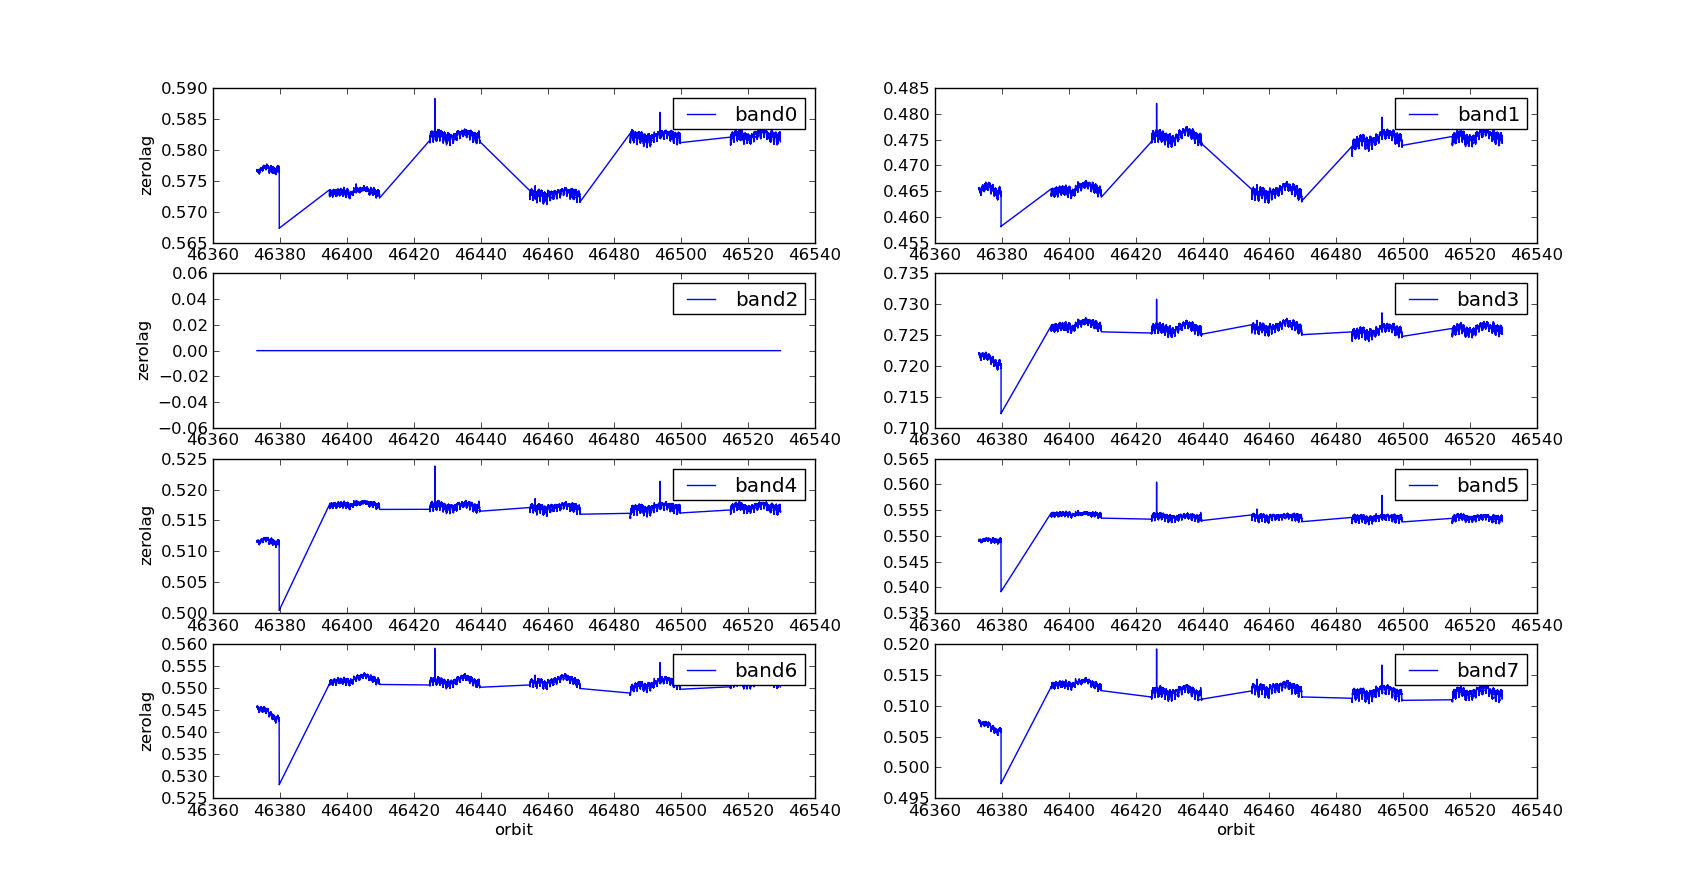
\includegraphics[scale=0.35]{ac2zerolag.png}\\
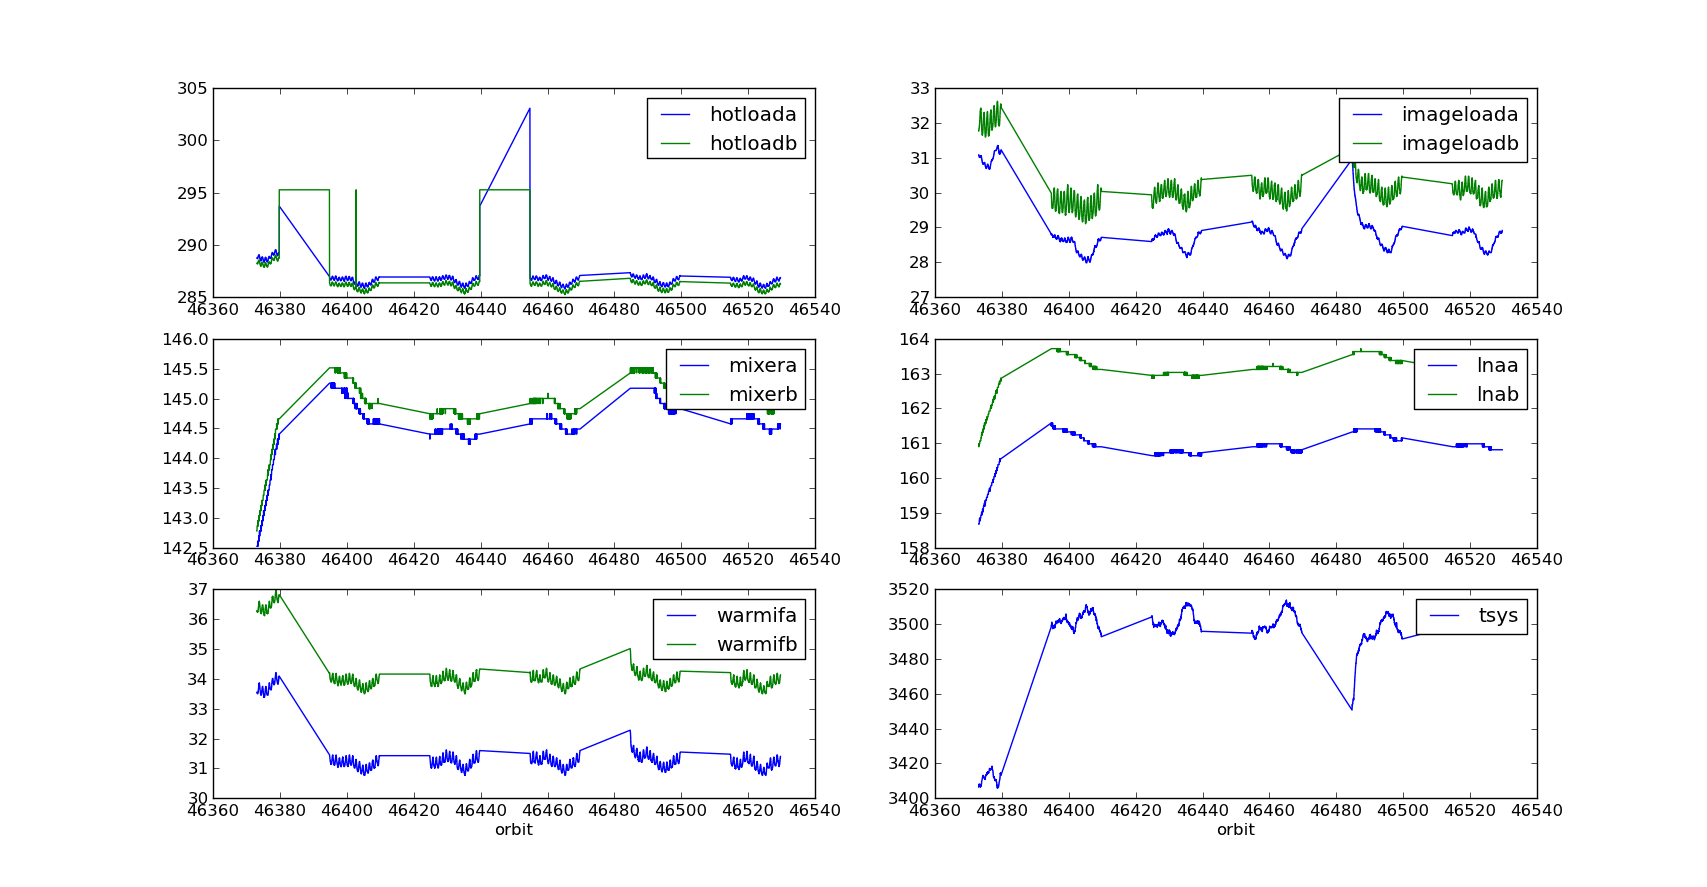
\includegraphics[scale=0.35]{ac2temp.png}\\
\caption{The upper panels show zerolags for the sky beam from AC2 
(stratospheric 1 mode)
for around 100 orbits. The lower panels show temperature information.}
\label{fig:study1ac2a}
\end{figure}

\begin{figure}[!t]
\centering
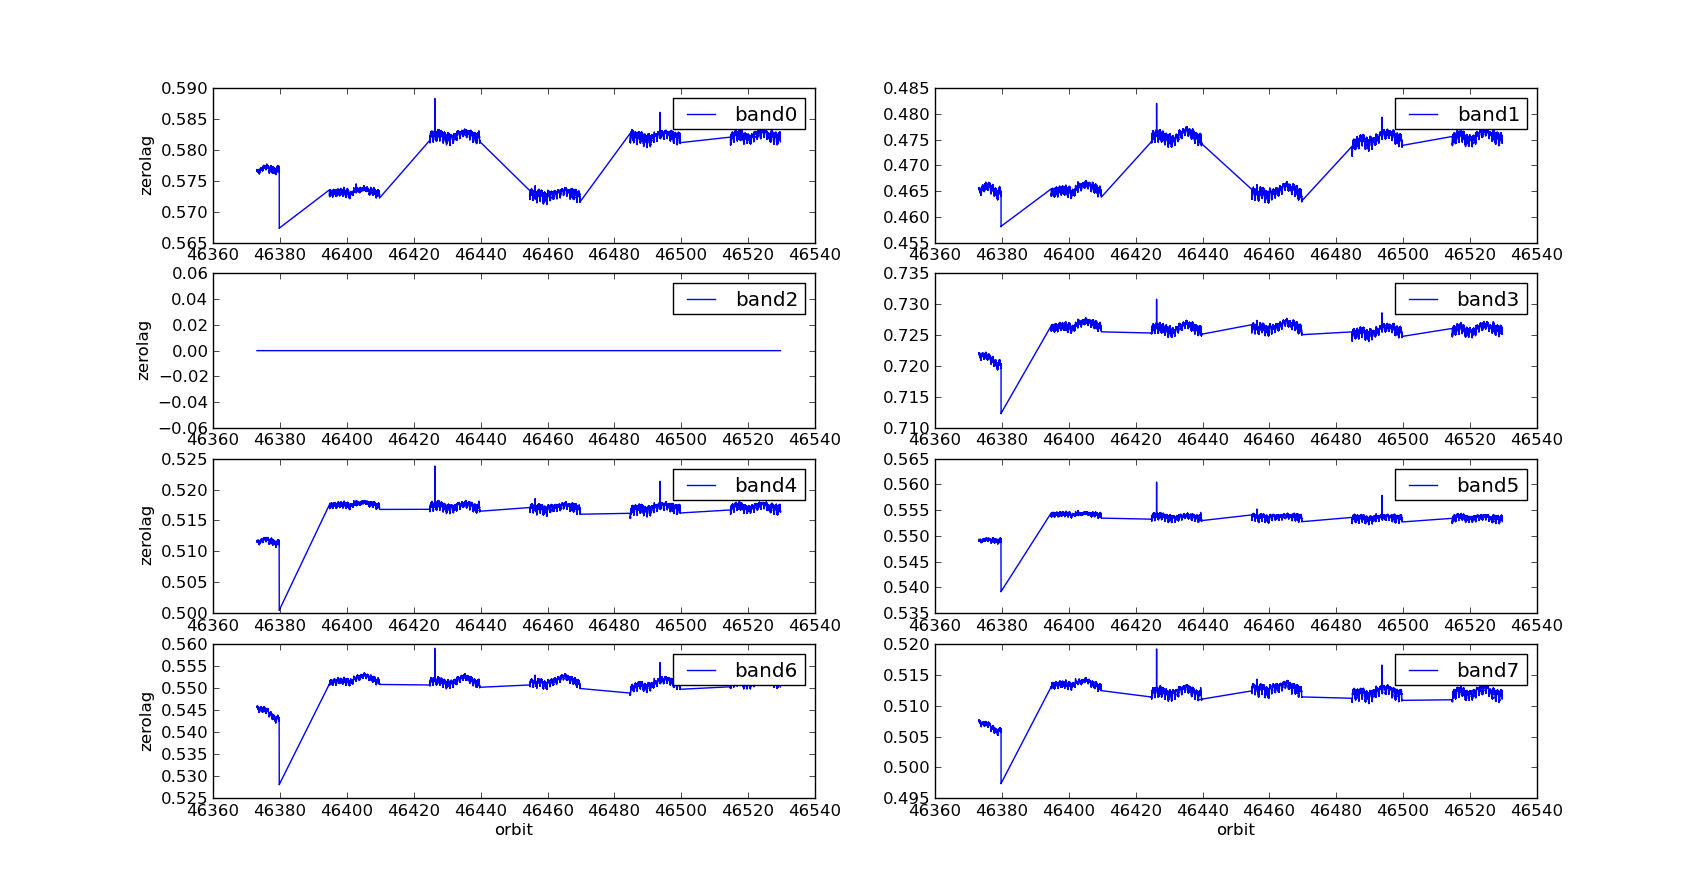
\includegraphics[scale=0.35]{ac2zerolag.png}\\
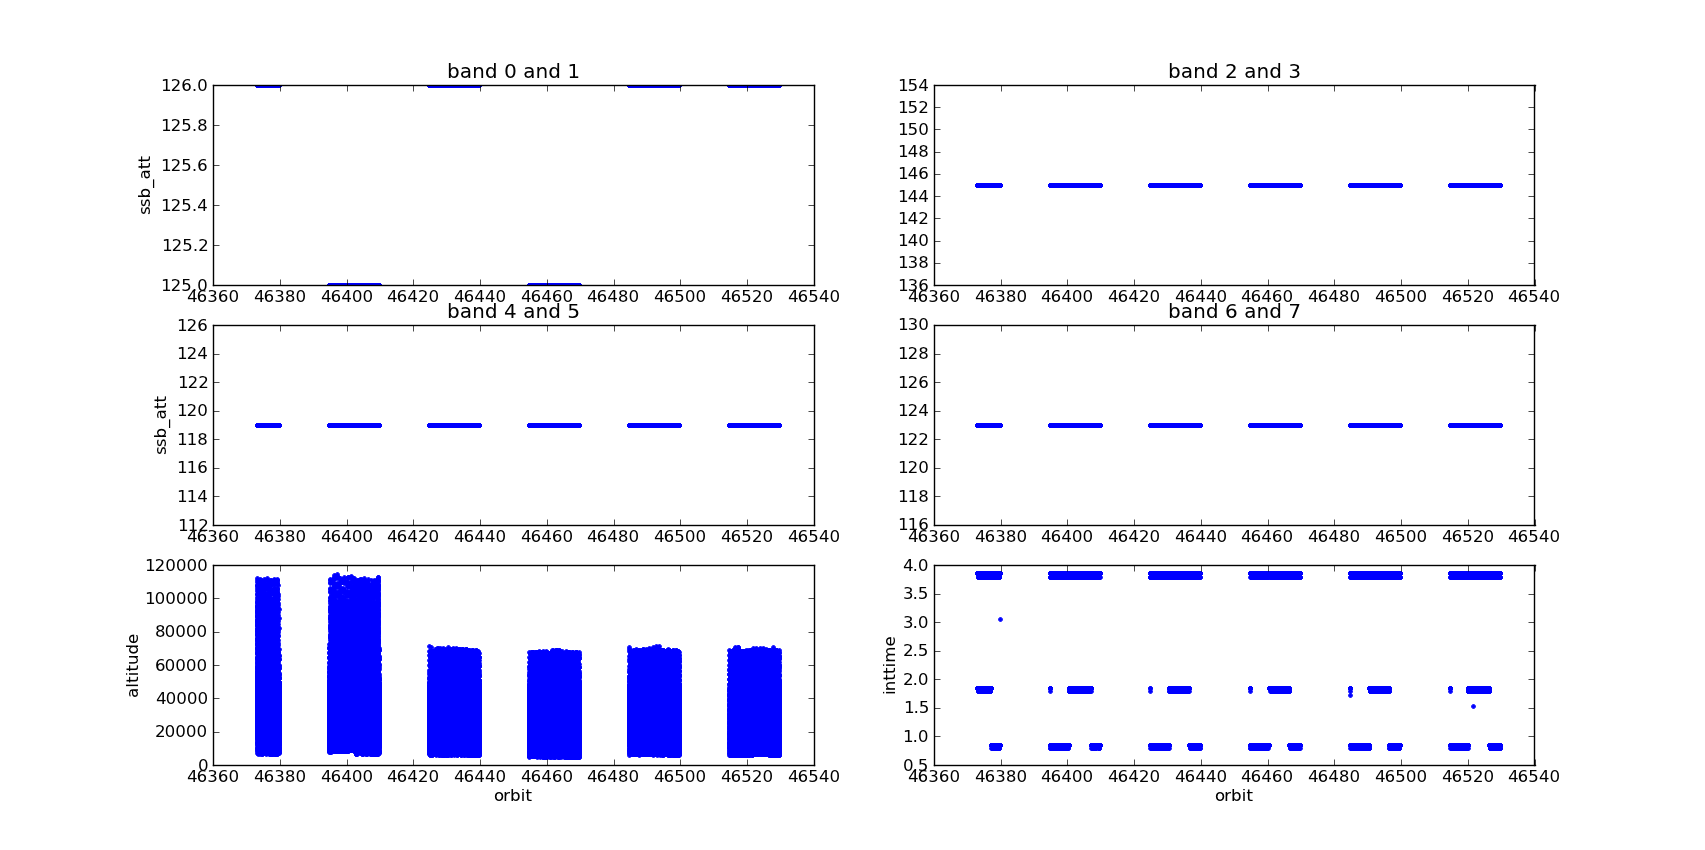
\includegraphics[scale=0.35]{ac2ssbatt.png}\\
\caption{The upper panels show zerolags for the sky beam from AC2 
(stratospheric 1 mode)
ssb-attenuators settings, altitudes, and integration times
matching Fig.~\ref{fig:study1ac2a}.}
\label{fig:ac2b}
\end{figure}

\begin{figure}[!t]
\centering
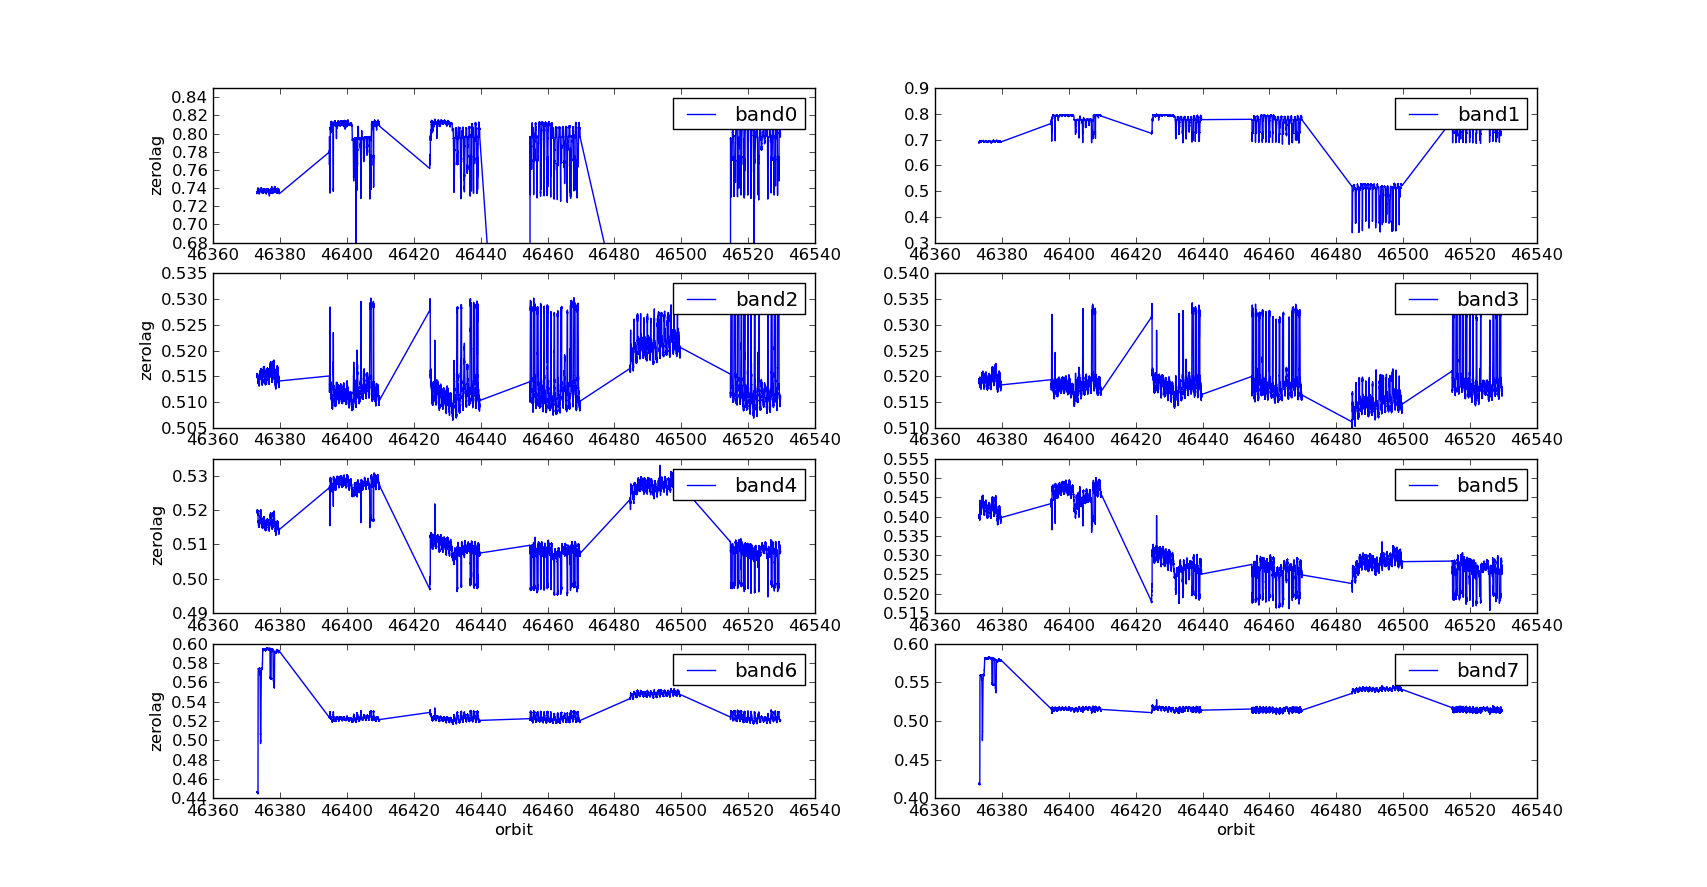
\includegraphics[scale=0.35]{ac1zerolag.png}\\
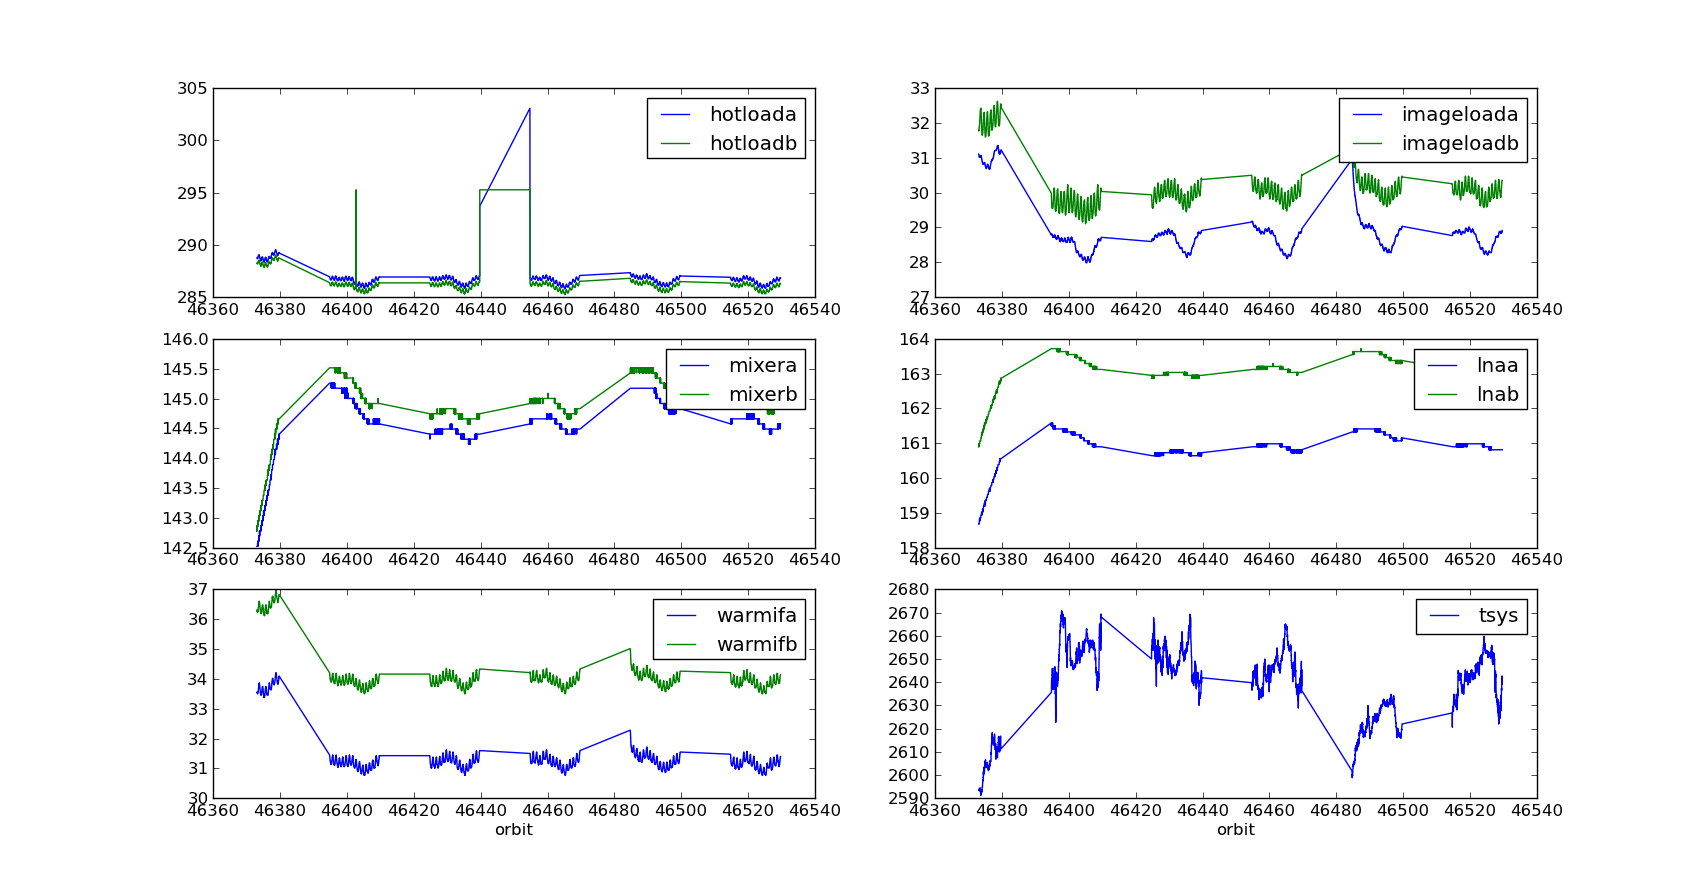
\includegraphics[scale=0.35]{ac1temp.png}
\caption{The upper panels show zerolags for the sky beam from AC1 
(stratospheric 2 mode)
for around 100 orbits. The lower panels show temperature information.}
\label{fig:study1ac1a}
\end{figure}

\begin{figure}[!t]
\centering
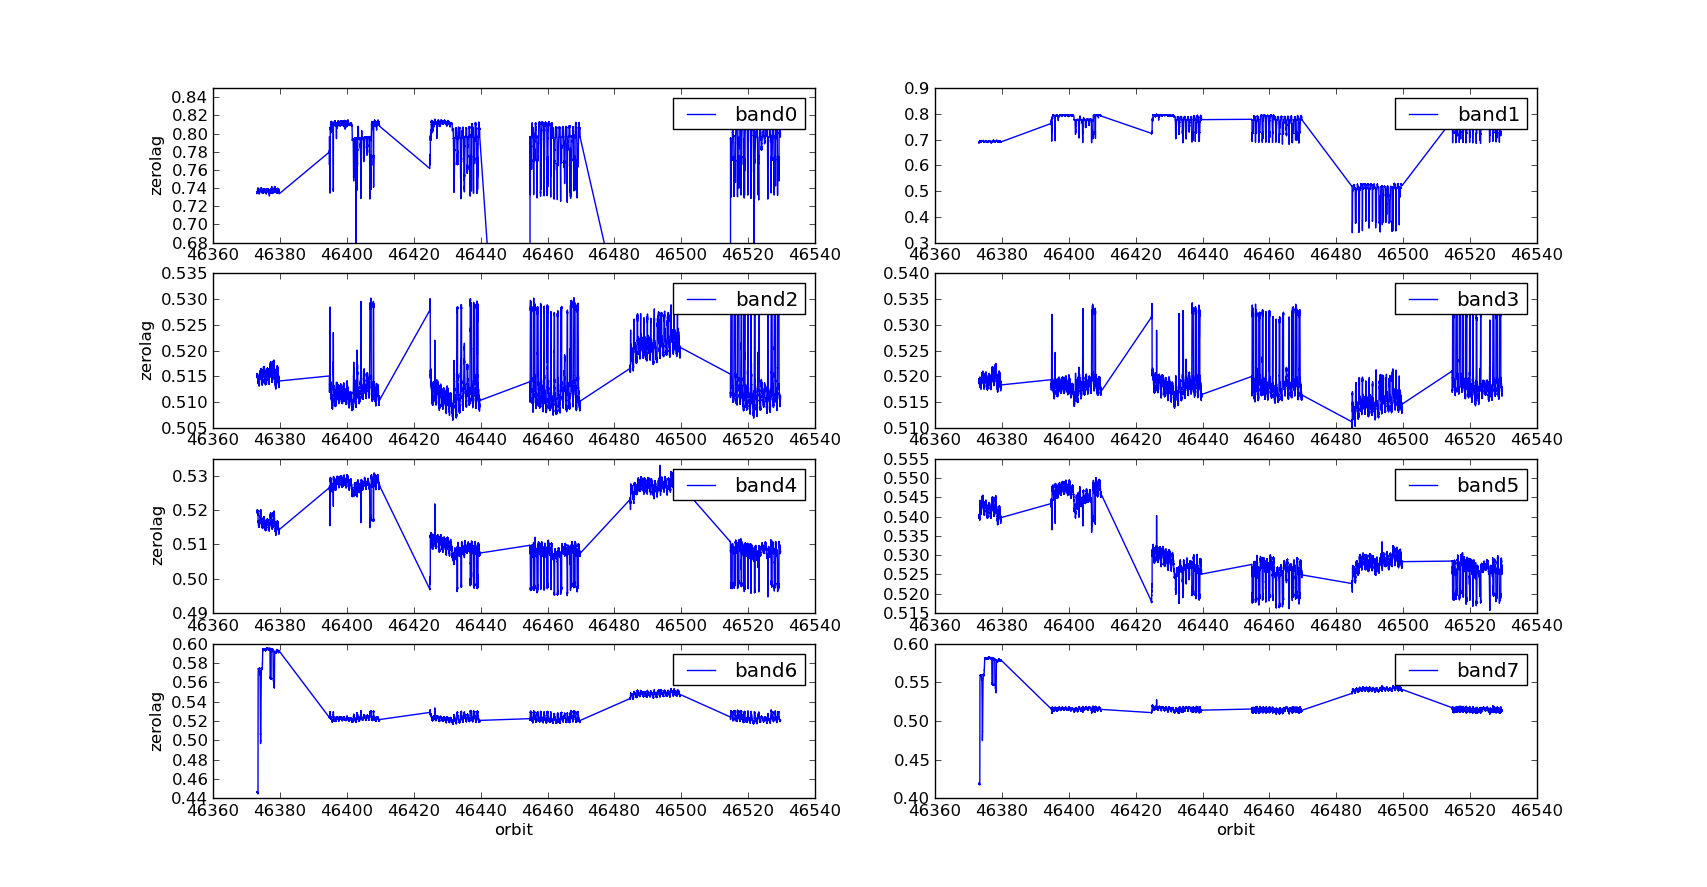
\includegraphics[scale=0.35]{ac1zerolag.png}\\
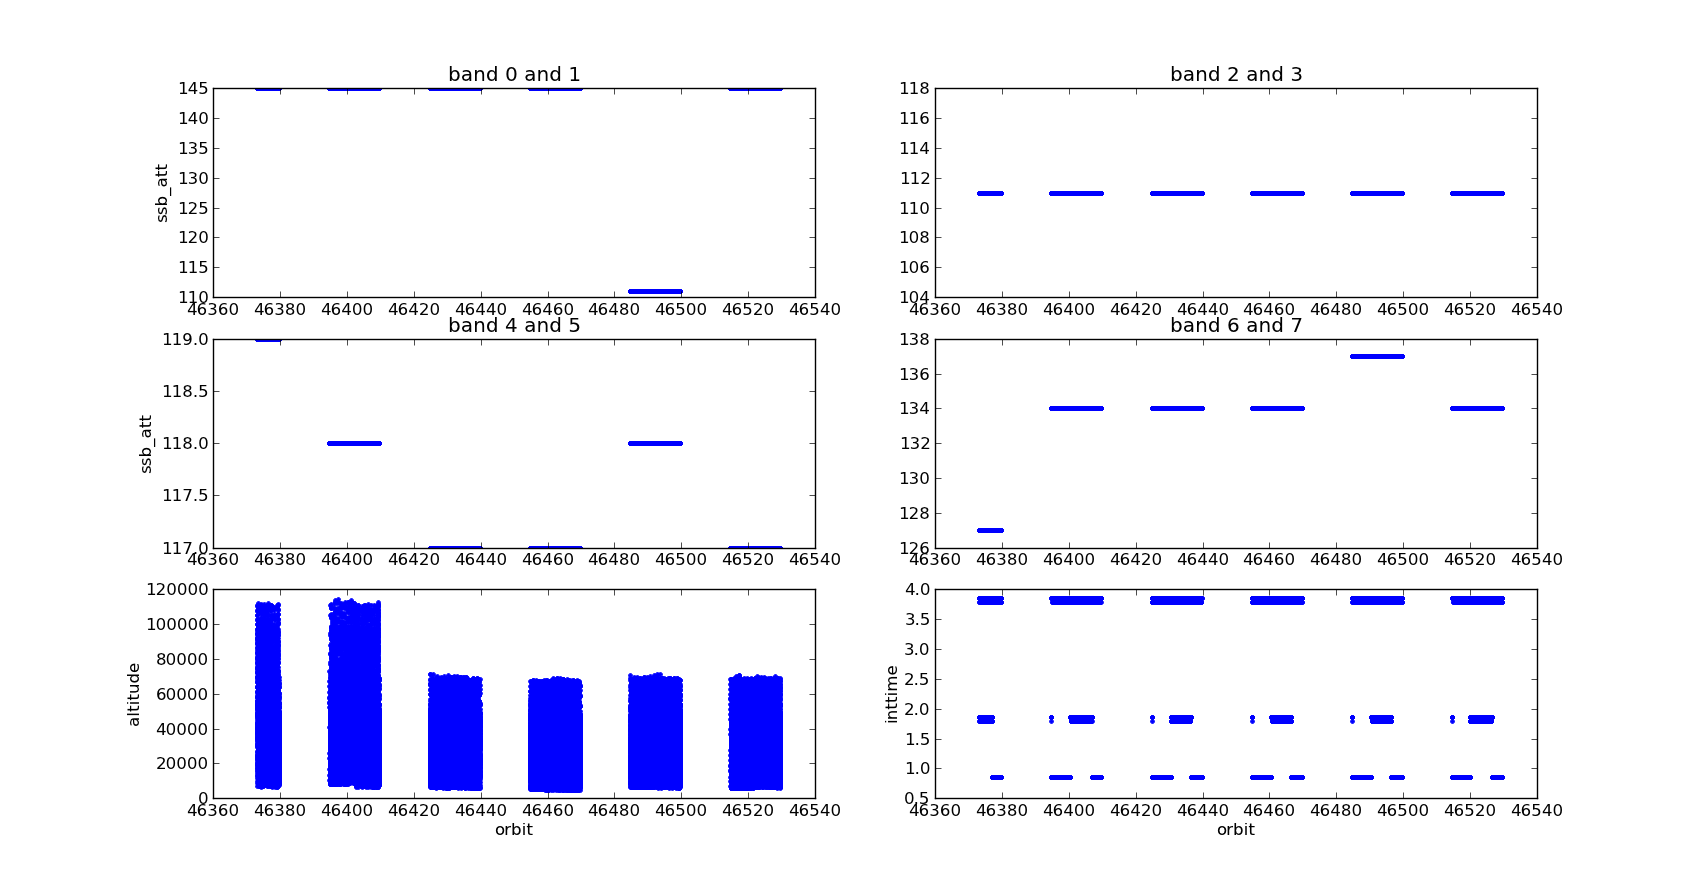
\includegraphics[scale=0.35]{ac1ssbatt.png}\\
\caption{ssb-attenuators settings, altitudes, and integration times
matching Fig.~\ref{fig:study1ac1a}.}
\label{fig:study1ac1b}
\end{figure}

%%%%%
\begin{figure}[!t]
\centering
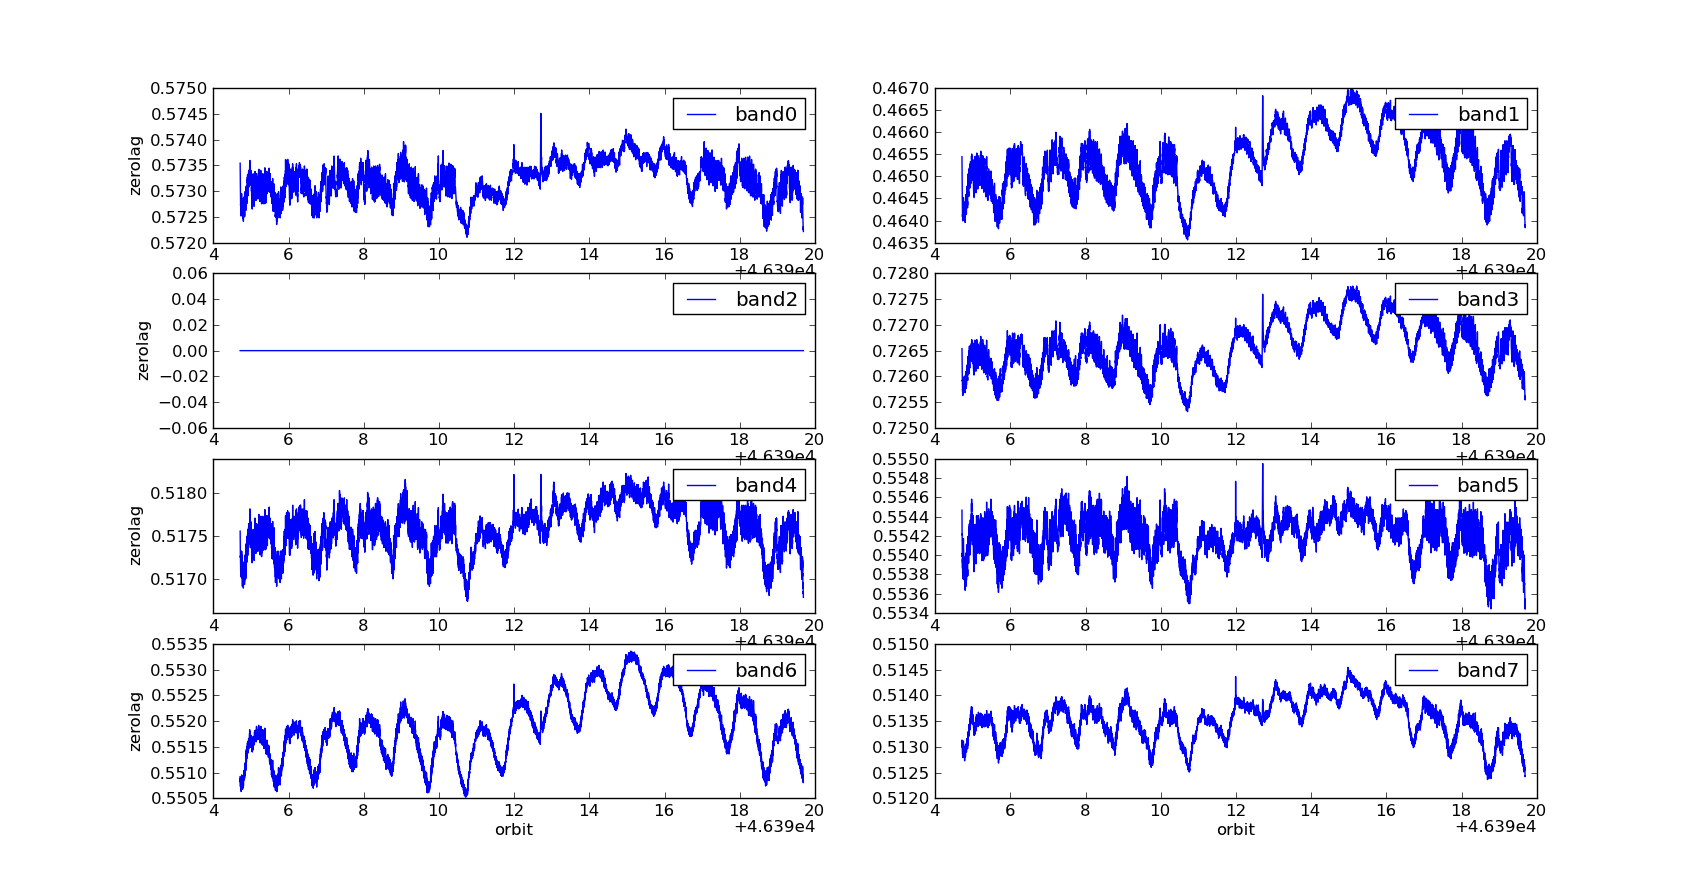
\includegraphics[scale=0.35]{ac2zerolag20orbits.png}\\
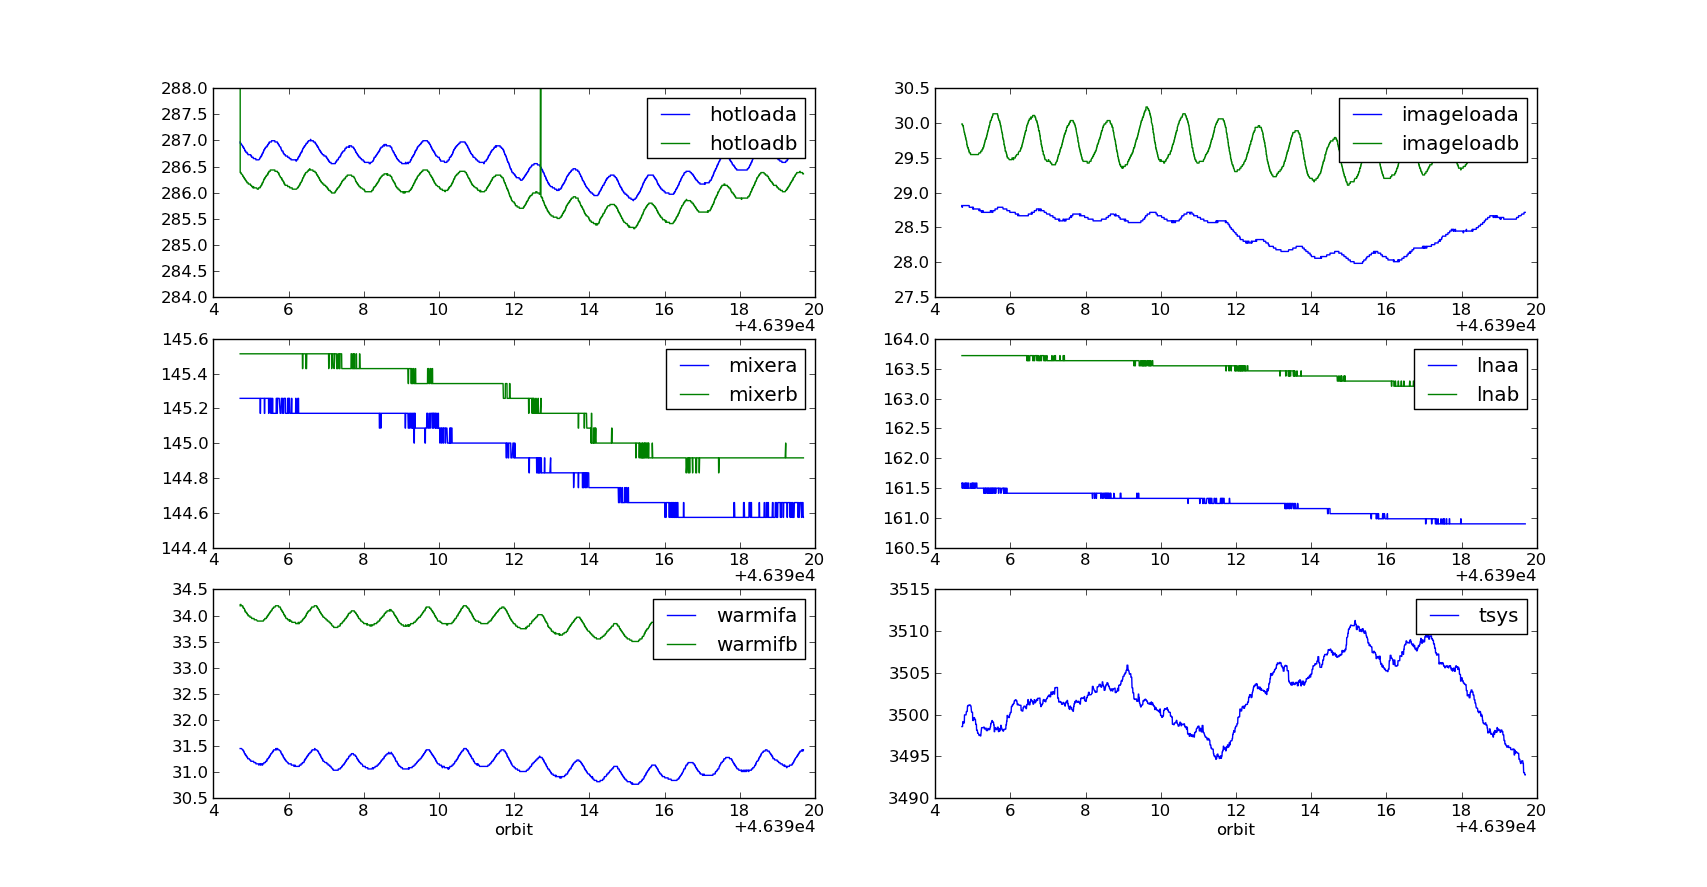
\includegraphics[scale=0.35]{ac2temp20orbits.png}\\
\caption{The upper panels show zerolags for the sky beam from AC2 
(stratospheric 1 mode)
for around 20 orbits. The lower panels show temperature information.}
\label{fig:study1ac2c}
\end{figure}

\begin{figure}[!t]
\centering
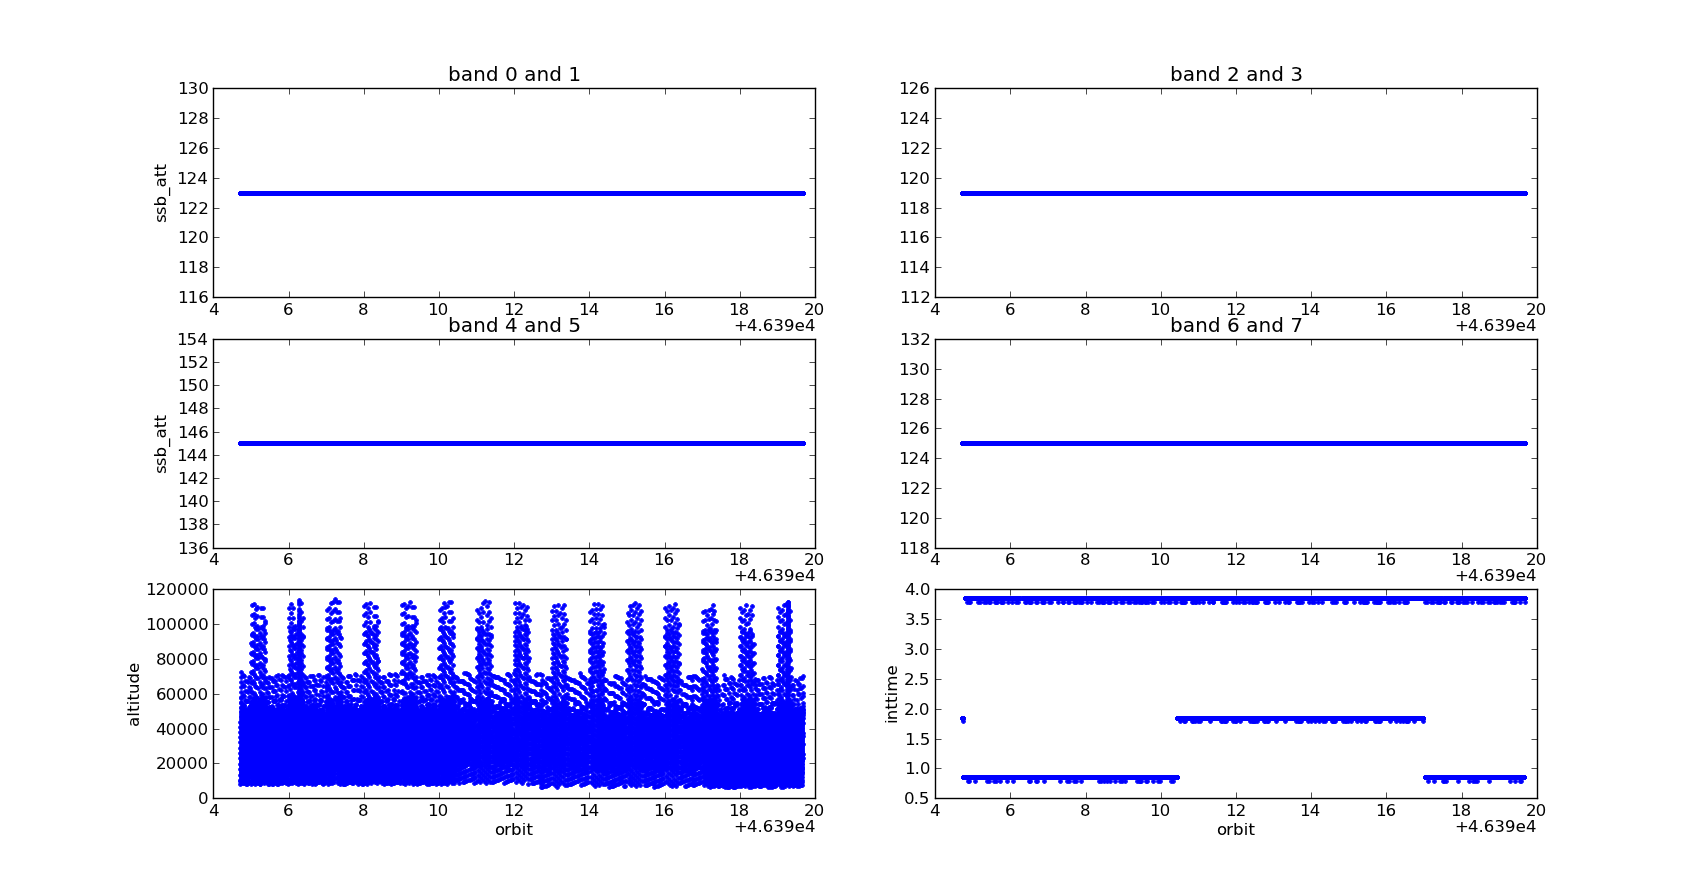
\includegraphics[scale=0.35]{ac2ssbatt20orbits.png}
\caption{ssb-attenuators settings, altitudes, and integration times
matching Fig.~\ref{fig:study1ac2c}.}
\label{fig:study1ac2d}
\end{figure}

\begin{figure}[!t]
\centering
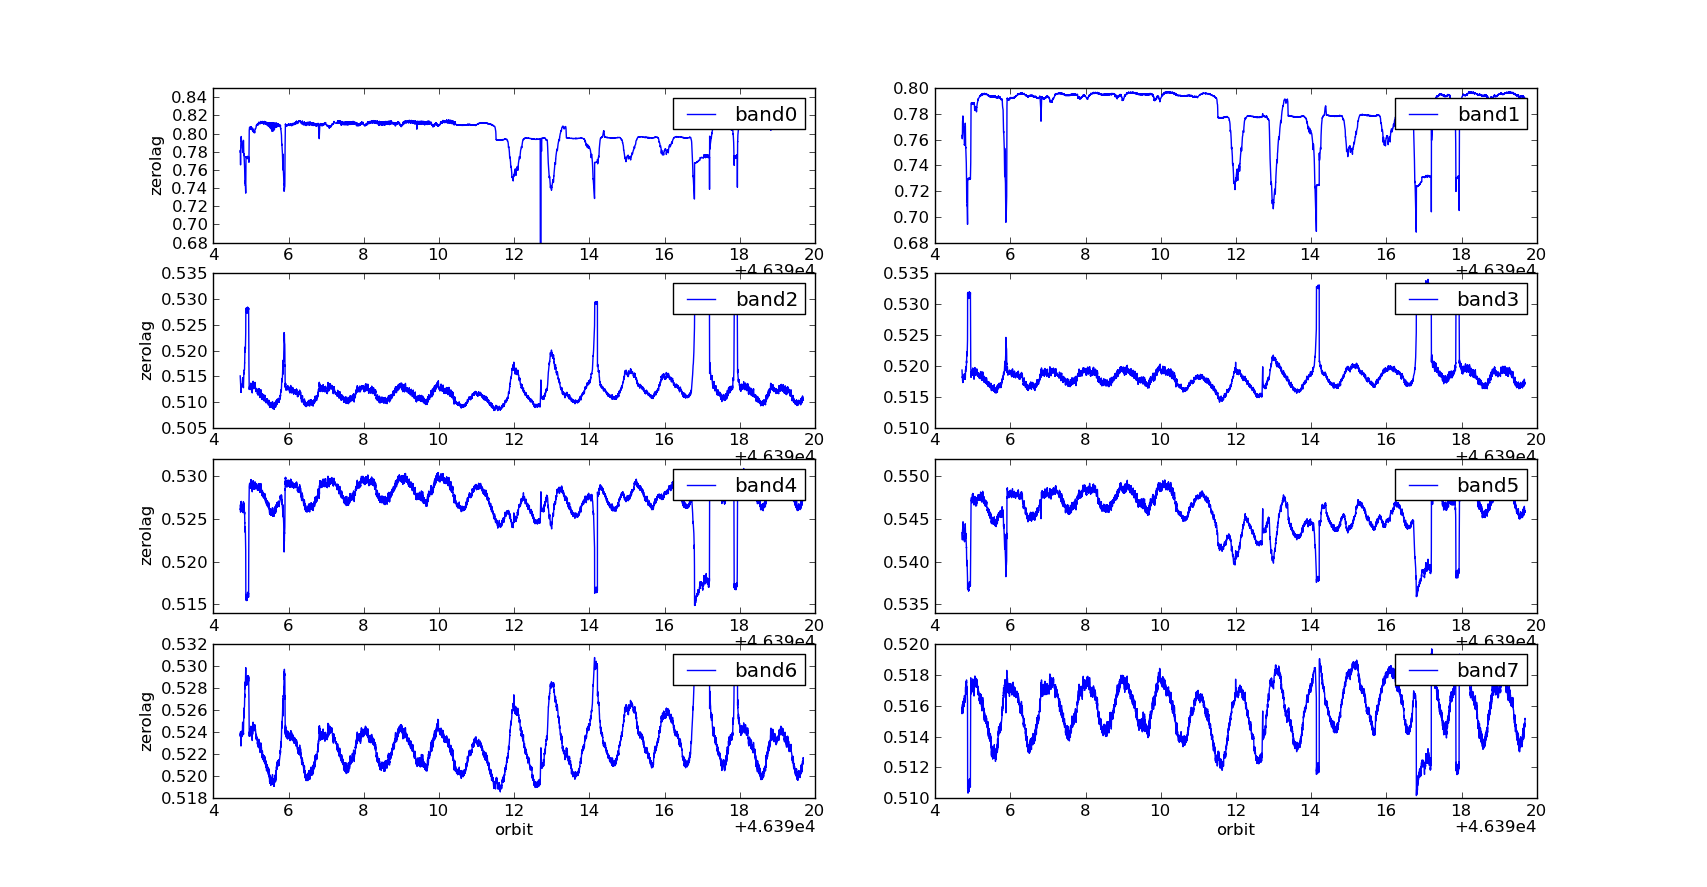
\includegraphics[scale=0.35]{ac1zerolag20orbits.png}\\
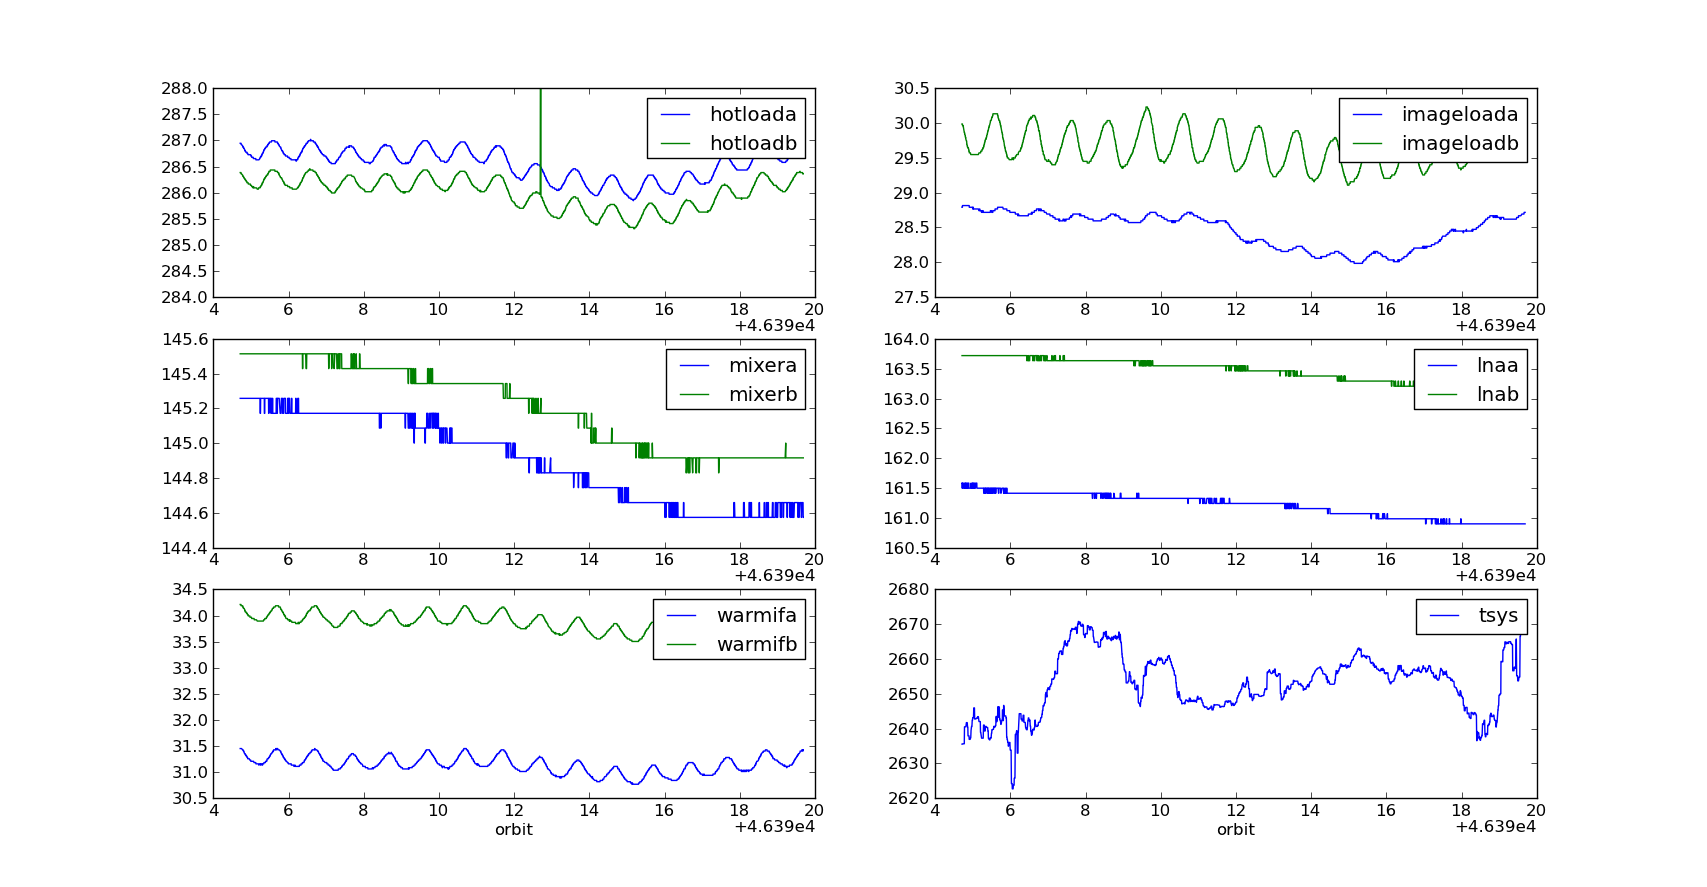
\includegraphics[scale=0.35]{ac1temp20orbits.png}
\caption{The upper panels show zerolags for the sky beam from AC1 
(stratospheric 2 mode)
for around 20 orbits. The lower panels show temperature information.}
\label{fig:study1ac1c}
\end{figure}

\begin{figure}[!t]
\centering
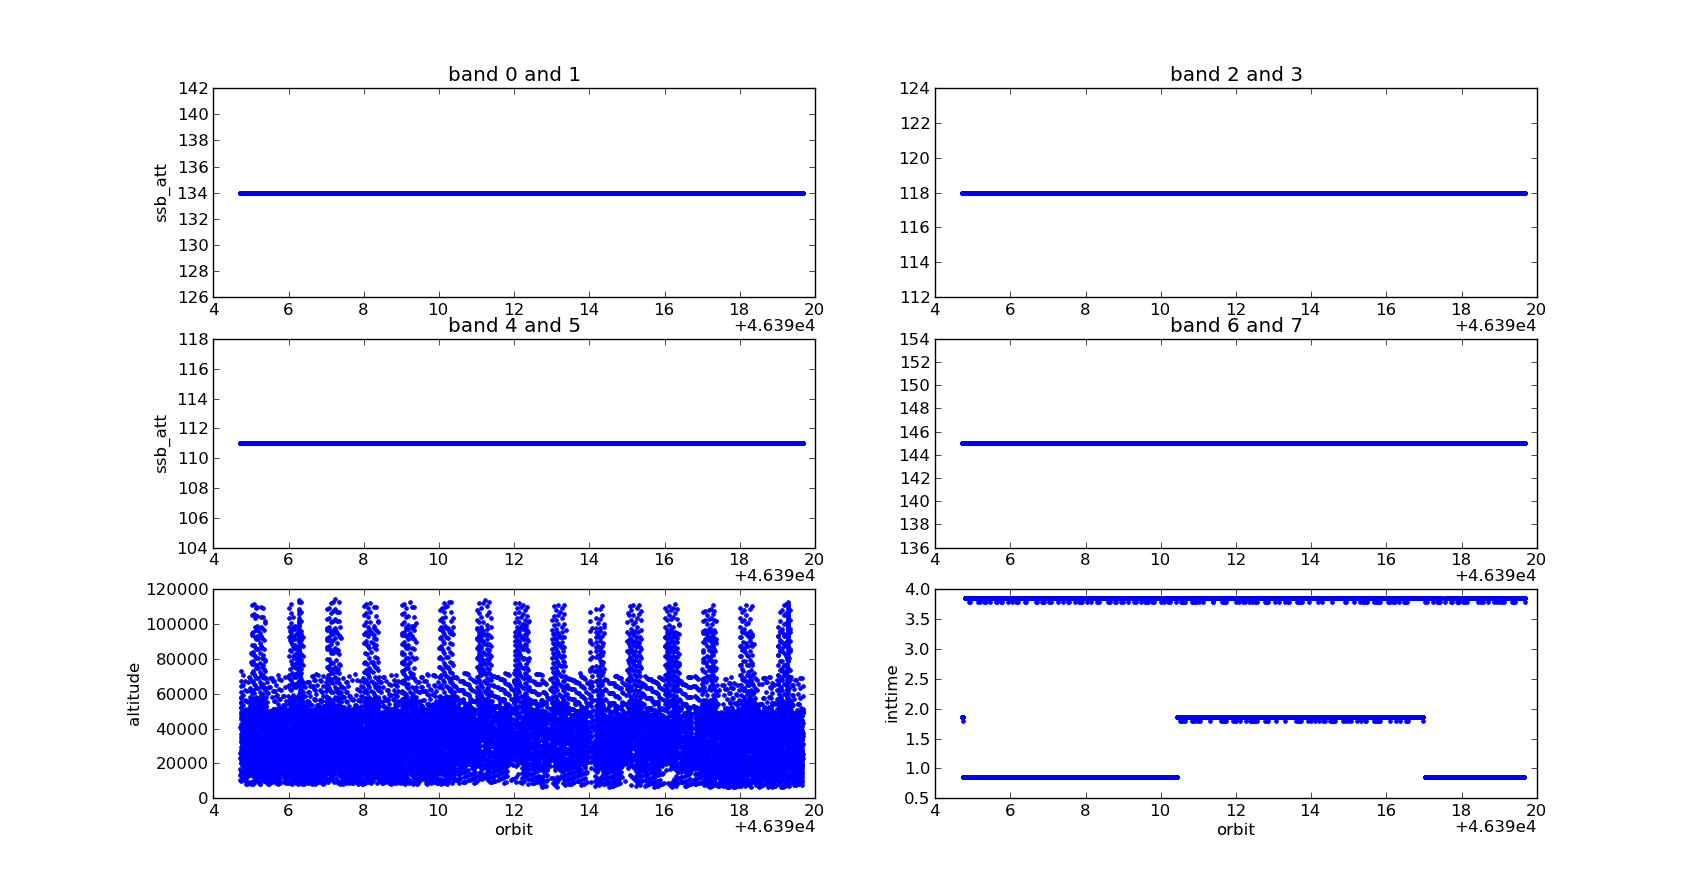
\includegraphics[scale=0.35]{ac1ssbatt20orbits.png}
\caption{ssb-attenuators settings, altitudes, and integration times
matching Fig.~\ref{fig:study1ac1c}.}
\label{fig:study1ac1d}
\end{figure}

We have earlier seen that we have variations in the zerolag
levels for the various bands of AC1 and AC2 that we want to
understand better. In the following figures zerolags
are plotted together with various temperature information
(more than we have shown earlier)
as function of orbit.
From Figures~\ref{fig:study1ac2a} and ~\ref{fig:study1ac1a},
which shows zerolags from AC2 and AC1 for around 100 orbits,
we can see that AC2 is more stable than AC1. 
The zerolgas of AC2 seems to be fairly stable for each period
of observation, even though the level can differ between different
periods (see band 0 and band 1 in Figure~\ref{fig:study1ac2a}).
This latter variation can not easily be explained by the temperature
information we have.

From Figures~\ref{fig:study1ac2c} and ~\ref{fig:study1ac1c}
which show zerolags from AC2 and AC1 for around 20 orbits
(a period where the observation modes were not changed),
it can be seen that AC2 zerolags are correlated to various
temperatures. When temperature is relatively high zerolags are
relatively low and vice versa.
Even AC1 zerolags show this pattern, but for some periods of time
the levels of zerolags changes in a way that we do not see from AC2.
Figure~\ref{fig:study1ac1c} shows also that the level of zerolag of each band 
of AC1 can occasionally change. 

\clearpage
\newpage
\section{High altitude spectra}
\begin{figure}[!t]
\centering
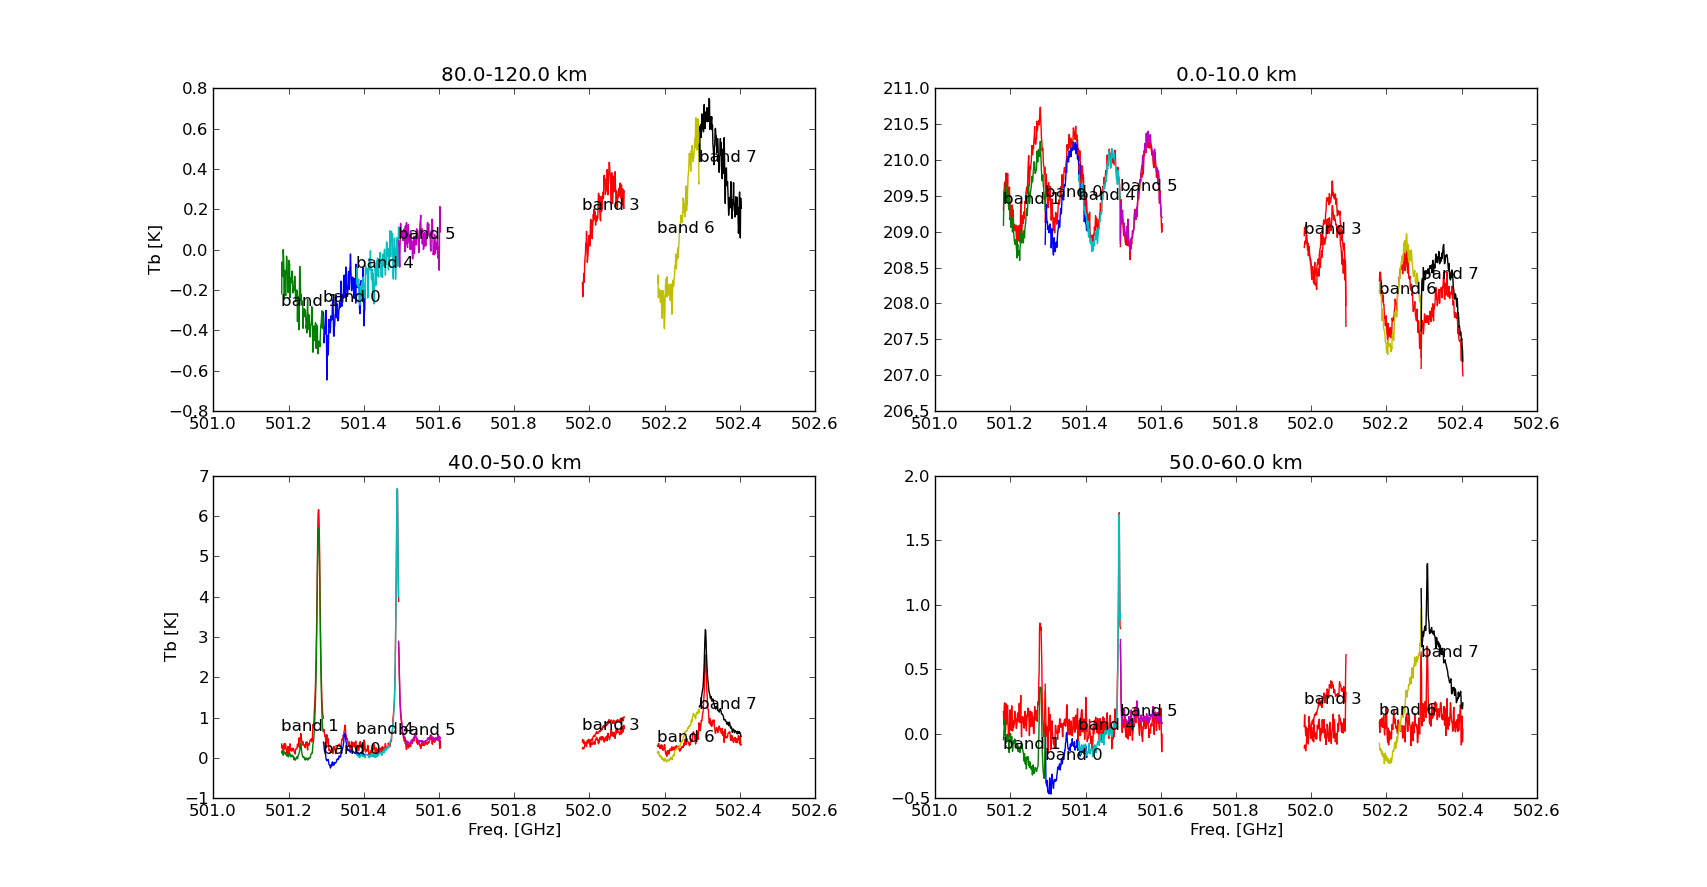
\includegraphics[scale=0.35]{ac2corr.png}
\caption{Calibrated data from AC2. The upper left panel shows
the median of measurents between 80-120 km. The other panels contain
both the mean of calibrated spectra between the heights in the title
of panels, and a spectrum (red) where the median of measurents between 80-120 km
has been subtracted. }
\label{fig:study1ac2corr}
\end{figure}


\begin{figure}[!t]
\centering
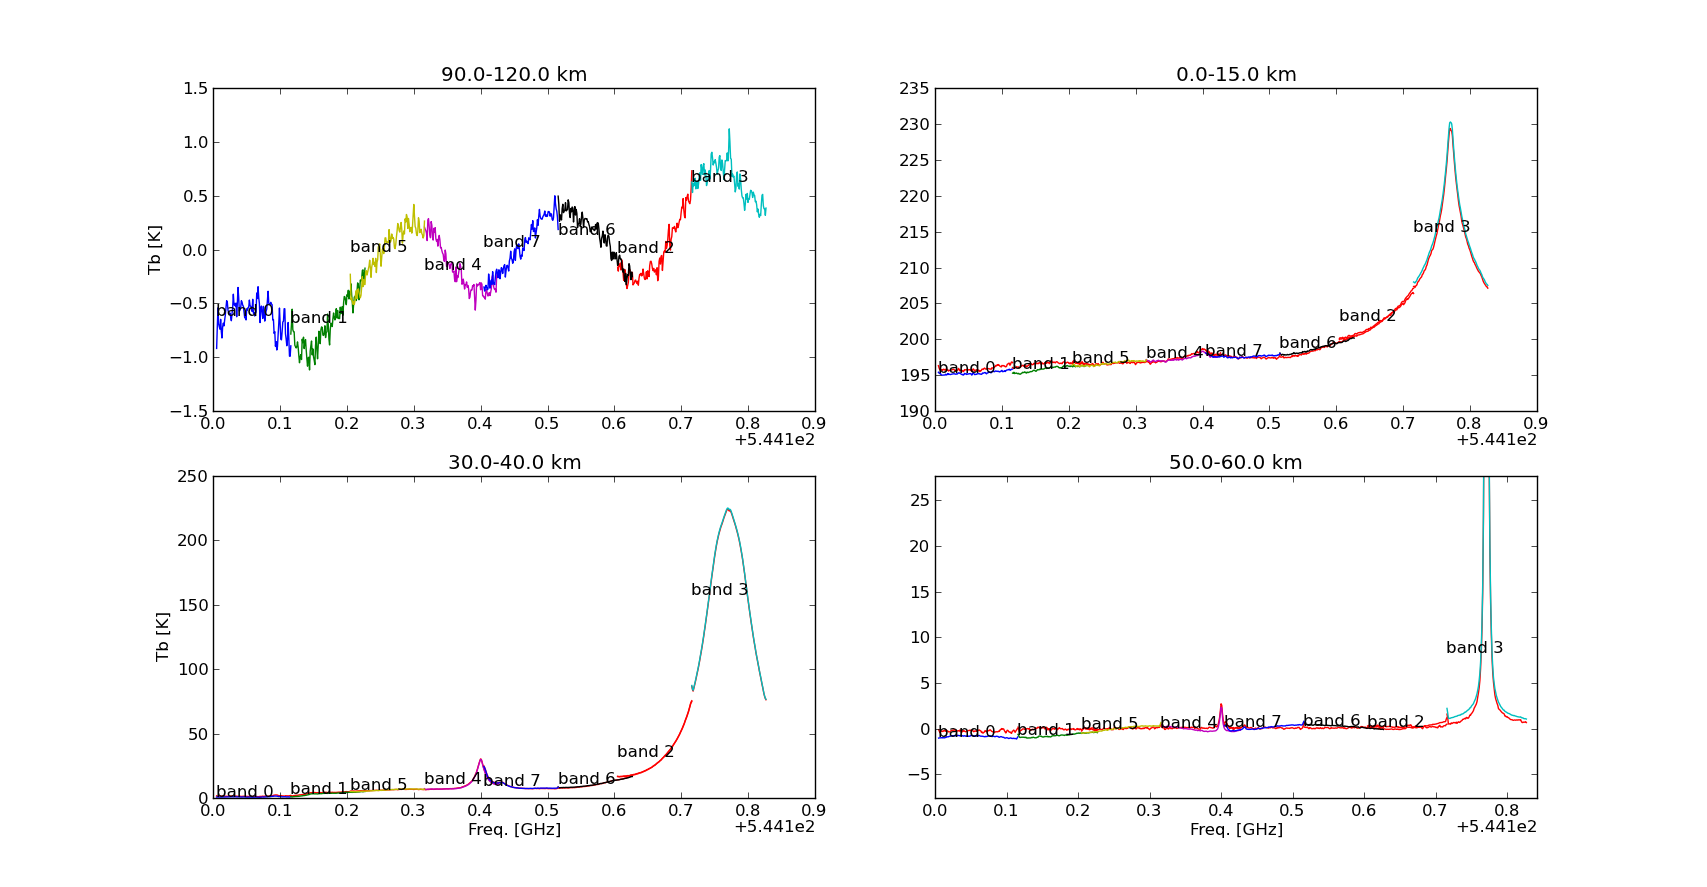
\includegraphics[scale=0.35]{ac1corr.png}
\caption{Calibrated data from AC2. The upper left panel shows
the median of measurents between 90-120 km. The other panels contain
both the mean of calibrated spectra between the heights in the title
of panels, and a spectrum (red) where the median of measurents between 90-120 km
has been subtracted.}
\label{fig:study1ac1corr}
\end{figure}
    
We know from earlier calibration versions of AC data from Odin-SMR
that high altitude spectrum, where we do not expect any spectral
feature, do contain a spectral feature. 

We have calibrated data from around 100 orbits where we have used
a slightly new calibration scheme (a \(\pm\)45 min window instead
of orbit-based calibration and a harder filtering of data). 
 
Figures~\ref{fig:study1ac2corr} and ~\ref{fig:study1ac1corr} show average
results from this calibration. From the upper left panels in
both figures it can be seen that average spectra still contains
spectral fetaures. The spectral fetaure from AC1 and AC2 looks
distincly different.
However, the spectral feature we also see from measurements
at lower altitudes (except from AC2 data at really low altitudes
where we see something else). The spectral feature at high altitudes
should have it's
origin in the antenna and the optics. The calibration scheme as it is
only corrects for this by a constant value (the mean of the mean
of high altitude spectra is close to zero).
Figures~\ref{fig:study1ac2corr} and ~\ref{fig:study1ac1corr} show that if we
subtract the ``high altitude signal'' from measurements from lower
altitudes these spectra looks more flat where it should.
Thus, the high spectral feature can be calibrated away (removed) 
as a frequency dependent tspill contribution.  

\section{Calibration of sky signals}
As a healty check of the calibration routine we have calibrated 
sky signals (not using the target sky signal in the calibration
process). Figures ~\ref{fig:study1ac2skysig} and ~\ref{fig:study1ac1skysig}
show time series of calibrated sky signals (mean of each band). 
On average the sky signal is close to 0 k, but occasionally
and specially
when zerolags timeseries looks ``strange'' the signal
can differ significantly from 0 K (see Figure~\ref{fig:study1ac1skysig}).

The calibrated sky signals before a target atmospheric signal 
can serve as a quality flag.


\begin{figure}[!t]
\centering
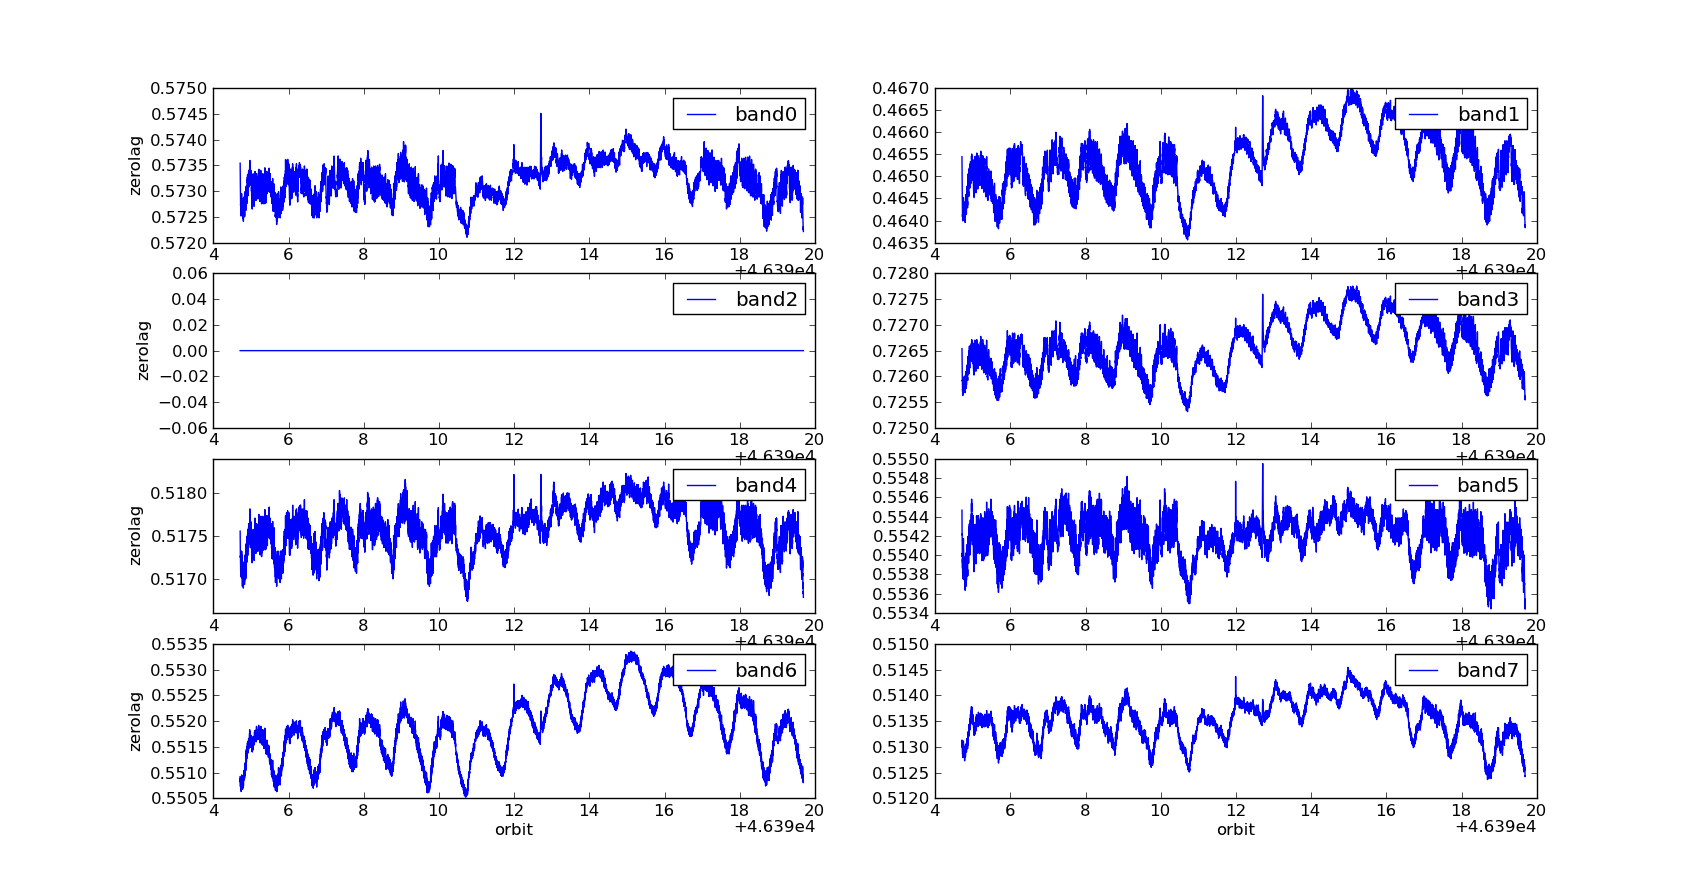
\includegraphics[scale=0.35]{ac2zerolag20orbits.png}
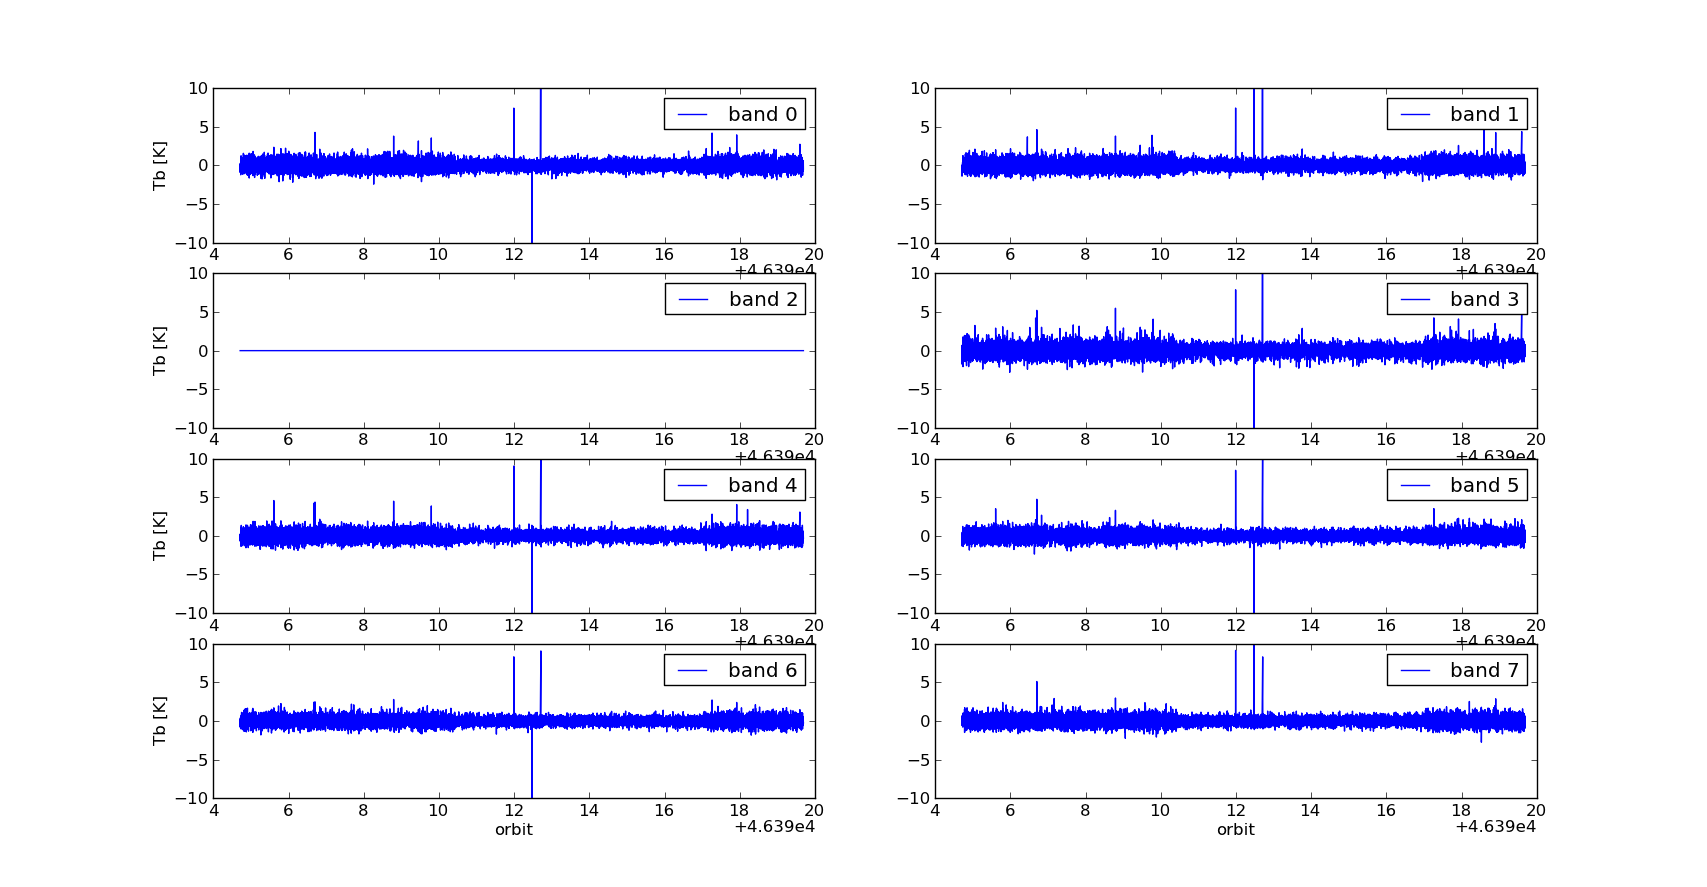
\includegraphics[scale=0.35]{ac2skysig.png}
\caption{The upper panels shows zerolags for AC2 (same as Figure~\ref{fig:study1ac2c}) and the lower panels shows the mean Tb of calibrated sky signals of each band.
}
\label{fig:study1ac2skysig}
\end{figure} 

\begin{figure}[!t]
\centering
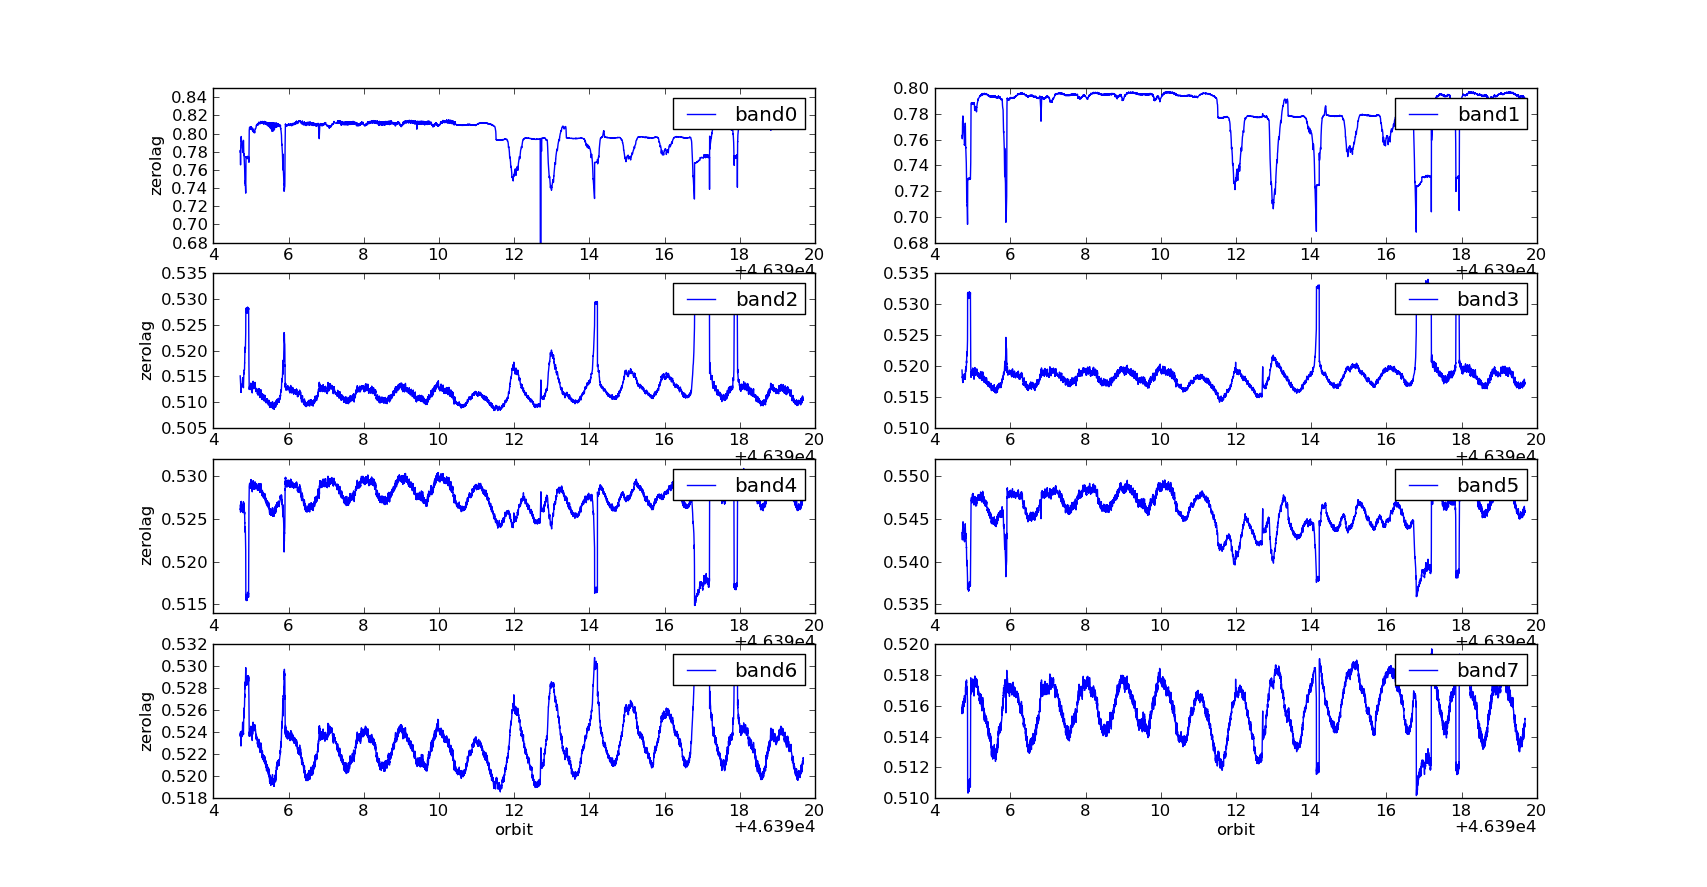
\includegraphics[scale=0.35]{ac1zerolag20orbits.png}
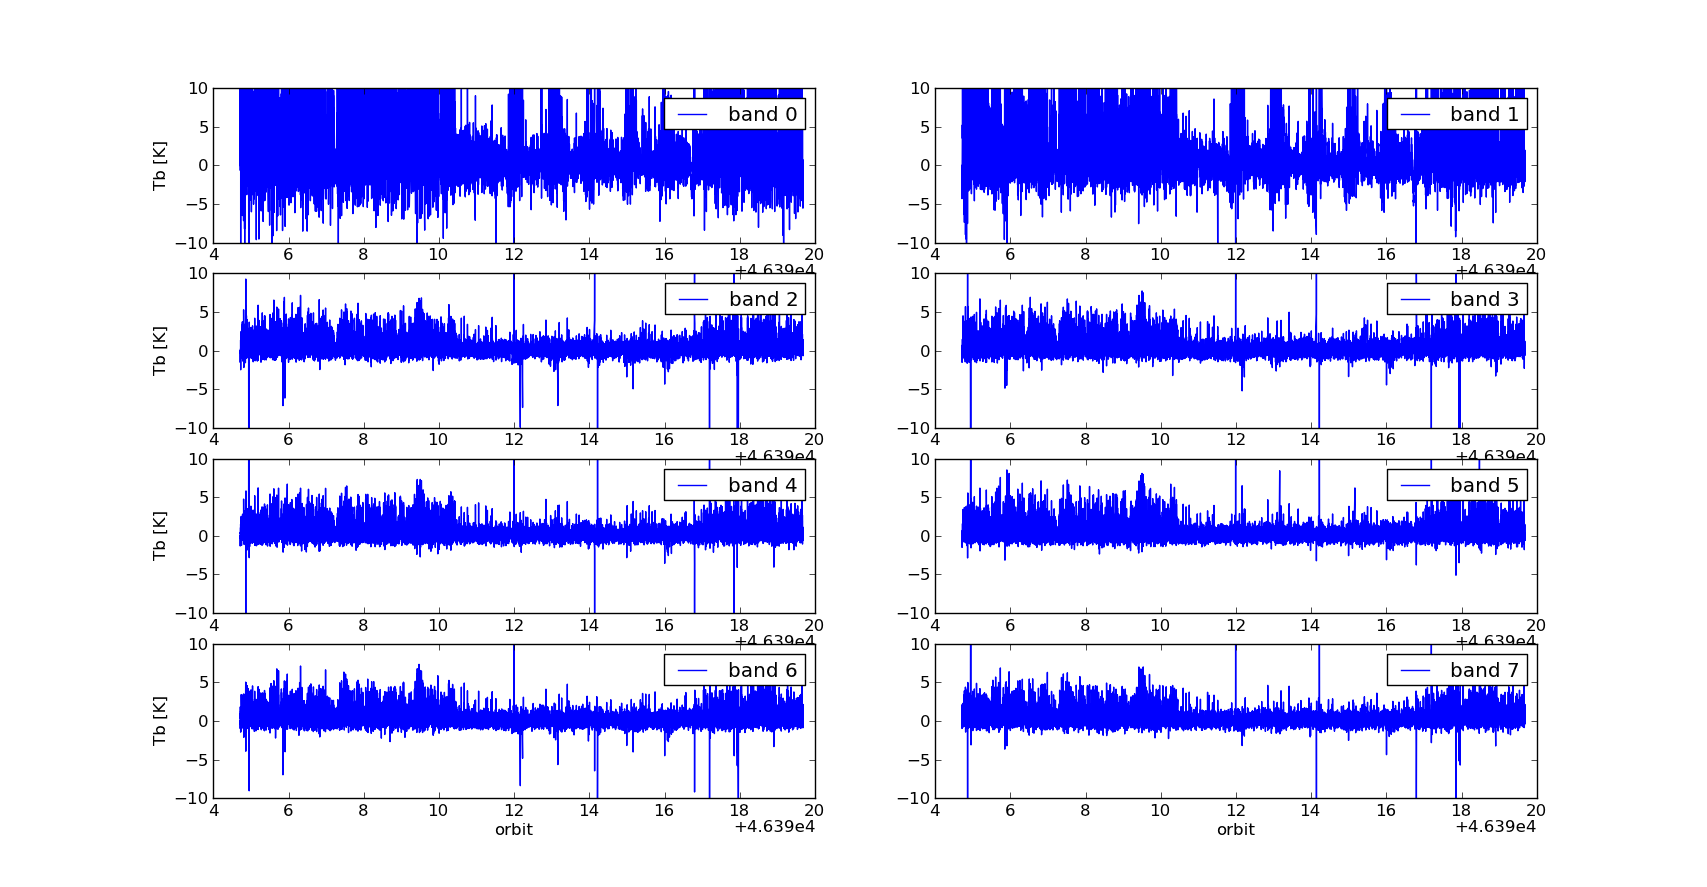
\includegraphics[scale=0.35]{ac1skysig.png}
\caption{The upper panels shows zerolags for AC1 (same as Figure~\ref{fig:study1ac1c}) and the lower panels shows the mean Tb of calibrated sky signal of each band.}
\label{fig:study1ac1skysig}
\end{figure} 


  
%%%%%%%%%%






